% Copyright (c) 2015 Luke Bowden and Callum O'Brien 

% Permission is granted to copy, distribute and/or modify this document under 
% the terms of the GNU Free Documentation License, Version 1.3 or any later 
% version published by the Free Software Foundation; with no Invariant Sections,
% no Front-Cover Texts, and no Back-Cover Texts. A copy of the license is 
% included in the file entitled "LICENSE.md".

\documentclass[draft]{book}

\usepackage{booktabs}

\usepackage{geometry}

\usepackage[toc]{glossaries}
\makeglossaries
\newglossaryentry{attribute} {
    name=attribute,
    description={a factor of some kind of entity}
}

\newglossaryentry{daemon} {
    name=daemon,
    description={A program or process that sits idly in the background until it
    is invoked to perform its task}
}

\newglossaryentry{database} {
    name=database,
    description={An organized collection of data. It is the collection of
    schemes, tables, queries, reports, views and other objects}
}

\newglossaryentry{entity} {
    name=entity,
    description={a thing in the modeled world},
    plural=entities
}

\newacronym{isbn}{ISBN}{International Standard Book Number}

\newglossaryentry{linux} {
    name=linux,
    description={A Unix-like and mostly POSIX-compliant computer operating
    system assembled under the model of free and open-source software
    development and distribution}, 
    plural=linuces
}

\newacronym{nfc}{NFC}{Near-Field Communication}

\newglossaryentry{posix} {
    name=POSIX,
    description={An acronym for Portable Operating System Interface, a family of
    standards specified by the IEEE Computer Society for maintaining
    compatibility between operating systems}
}

\newglossaryentry{record} {
    name=record,
    description={an item or collection of data}
}

\newglossaryentry{table} {
    name=table,
    description={A collection of related data held in a structured format within
    a database.} 
}

\newacronym{uid}{UID}{Unique Identifier}

\newglossaryentry{unix} {
    name=unix,
    description={a family of multitasking, multiuser computer operating systems
    that derive from the original AT\&T Unix, developed in the 1970s at the Bell
    Labs research center by Ken Thompson, Dennis Ritchie, and others},
    plural=unices    
}




\usepackage{listings}
\lstset{language=c}

\usepackage[round]{natbib}
\bibliographystyle{plainnat}

\usepackage{tabu}

\usepackage{tikz}

\begin{document}

\frontmatter

\title{Improving the EMS Library}
\author{Luke Bowden \& Callum O'Brien\\
    Exeter Mathematics School}
\date{\today}
\maketitle

\tableofcontents

\mainmatter

\chapter{Details and Context}

\section{Description of the Current System}

Exeter Mathematics School's library contains, as one might expect, books. Some
of the books are available to check out of the library, whereas others are
not; currently, this is communicated by stickers on the books with a grey
sticker on the spine of a book meaning one is not to take that book out of the
library. Other colour stickers of books' spines mean one can check them out.

When a student checks out a book, they write their name in a log book, along
with the current date. Upon returning the book, they find the entry in the log
book corresponding to its checking out and add the date they returned it. If
one wishes to find out who has a book or, indeed, whether a book is currently
in the library (without visually searching the shelves), one must read through
this log book, find the lastest entry regarding the book one wishes to know
about and see who checked it out and/or whether the book has been returned.

\section{Inefficiencies Arising from the Current System}

\section{Potential Solutions to Current Inefficiencies}

\section{Appraisal of Potential Solutions}

%%%%%%%%%%%%%%%%%%%%%%%%%%%%%%%%%%%%%%%%%%%%%%%%%%%%%%%%%%%%%%%%%%%%%%%%%%%%%%%%

\chapter{Design}

\section{Overall System Design}

The proposed system involves (as well as the obvious) a daemon, a database
and an NFC reader. Upon checking out a book, a student will touch both the
book and their identification card to an NFC reader device. This will invoke
the daemon which will query the Book and Student tables in the database for
the UIDs of the book and the student. After these data have been retrieved,
the daemon will query the database again, this time concerning the BookStudent
table; the daemon requests the UIDs of any BookStudent records whose BookID
and StudentID attributes are the recently retrieved UIDs and whose pending
attribute is True. This query will return either nothing or a single UID. If
no UID is received, the daemon will create a new record in the BookStudent
table. This record will have;\begin{itemize}

    \item BookID of the Book's UID
    \item StudentID of the Student's UID
    \item OutTime of the current time
    \item InTime of NULL
    \item Pending of True

\end{itemize} If a UID is received, the record with that UID is updated to
have;\begin{itemize}

    \item InTime of the current time
    \item Pending of False

\end{itemize}

\section{Entity Relationships \& Database Structure}

The database must encapsulate two entities, Book and Student, the Book entity
being an abstraction of a book in the EMS library and the Student entity being
an abstraction of a student attending EMS. The Book entity must contain all
information one might wish to identify a book by; its author, isbn, subject
and title. However, each instance of this entity must be unique and so a fifth
attribute, a UID, is required. The Student entity has attributes name and UID.

\begin{table}[t]

    \centering

    \begin{tabu} to 0.7\linewidth {lXX}

        \toprule

        Table       & Feild     & Type   \\

        \midrule

        Book        & Author    & Int    \\
                    & UID       & Int    \\
                    & ISBN      & String \\
                    & Subject   & String \\
                    & Title     & String \\

        BookStudent & BookID    & Int    \\
                    & InTime    & Date   \\
                    & OutTime   & Date   \\
                    & Pending   & Bool   \\
                    & StudentID & Int    \\
                    & UID       & Int    \\

        Student     & Name      & String \\
                    & UID       & Int    \\

        \bottomrule

    \end{tabu}

    \caption[Data Dictionary]{Tables and the fields they contain}

\end{table}

A single Student may take out many Books and a single Book may be taken out by
many Students, thus these entities have a many-to-many relationship. In order
to fully encapsulate these entities in a relational database we must normalise
this relationship, creating a third entity; BookStudent. A BookStudent record
will be created for every time a Student takes out a Book. This effects
a one-to-many relationship between Book and BookStudent and a many-to-one
relationship between BookStudent and Student (see figure 2.3).

\begin{figure}[b]

    \centering

    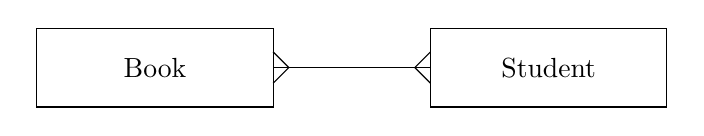
\begin{tikzpicture}

        % Book
        \draw (00.00,00.00) rectangle (03.00,01.00);
        \draw (01.50,00.50) node [text width=3cm, text centered] {Book};

        % Student
        \draw (05.00,00.00) rectangle (08.00,01.00);
        \draw (06.50,00.50) node [text width=3cm, text centered] {Student};

        % Book >-< Student
        \draw (03.00,00.50) -- (05.00,00.50);
        \draw (03.20,00.50) -- (03.00,00.70);
        \draw (03.20,00.50) -- (03.00,00.30);
        \draw (04.80,00.50) -- (05.00,00.70);
        \draw (04.80,00.50) -- (05.00,00.30);

    \end{tikzpicture}

    \caption[Unnormalised table structure]{The table structure of the 
        database before normalisation.}

\end{figure}

\begin{figure}[t]

    \centering

    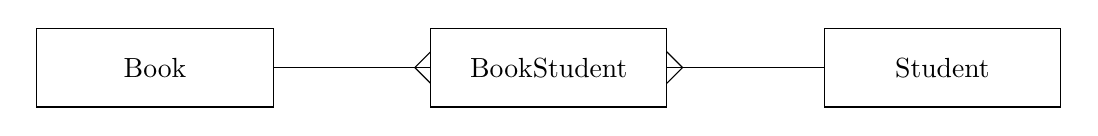
\begin{tikzpicture}

        % Book
        \draw (00.00,00.00) rectangle (03.00,01.00);
        \draw (01.50,00.50) node [text width=3cm, text centered] {Book};

        % BookStudent
        \draw (05.00,00.00) rectangle (08.00,01.00);
        \draw (06.50,00.50) node [text width=3cm, text centered] {BookStudent};

        % Student
        \draw (10.00,00.00) rectangle (13.00,01.00);
        \draw (11.50,00.50) node [text width=3cm, text centered] {Student};
       
        % Book -< BookStudent
        \draw (03.00,00.50) -- (5.00,0.50);
        \draw (04.80,00.50) -- (5.00,0.70);
        \draw (04.80,00.50) -- (5.00,0.30);

        % Student -< BookStudent
        \draw (08.00,00.50) -- (10.00,00.50);
        \draw (08.20,00.50) -- (08.00,00.70);
        \draw (08.20,00.50) -- (08.00,00.30);

    \end{tikzpicture}
    
    \caption[Normalised table structure]{The table structure of the database 
        after normalisation.}

\end{figure}

\section{User Interface}

\section{Security Measures}

%%%%%%%%%%%%%%%%%%%%%%%%%%%%%%%%%%%%%%%%%%%%%%%%%%%%%%%%%%%%%%%%%%%%%%%%%%%%%%%%

\chapter{Implementation}

\section{Discussion of Language}

\section{Discussion of Platform}

\section{Issues and Resolutions}

%%%%%%%%%%%%%%%%%%%%%%%%%%%%%%%%%%%%%%%%%%%%%%%%%%%%%%%%%%%%%%%%%%%%%%%%%%%%%%%%

\chapter{Testing}

%%%%%%%%%%%%%%%%%%%%%%%%%%%%%%%%%%%%%%%%%%%%%%%%%%%%%%%%%%%%%%%%%%%%%%%%%%%%%%%%

\chapter{Evaluation}

\section{Assessment of Features}

\section{Known Bugs}

\appendix

\chapter{Source Code}

\backmatter

\listoffigures

\listoftables

\bibliography{emc}

\printglossaries

\end{document}

